\chapter{Implementation}
\label{chap:implementation}
This chapter presents the implementation details of the proposed segmentation framework, as depicted in \figref{framework}. The primary goal of this chapter is to provide a comprehensive understanding of the practical aspects of this project. The subsequent sections discuss the specific components of the proposed segmentation framework, including \nameref{sec:programming_language}, \nameref{sec:deep_learning_framework}, \nameref{sec:experiment_management_tools}, the \nameref{sec:network_architecture} and a concise overview of a unique \nameref{sec:image_analysis_spreadsheet} utilized for an in-depth analysis of loss functions at the pixel level. To guarantee reproducibility and ease of use, the entire set of libraries and dependencies can be conveniently accessed within the provided Docker image this project includes and available on \href{https://github.com/MagicFeeling/framework-for-segmentation-loss-merging}{Github}. The repository's Readme file contains all the installation instructions for this work.

\section{Programming Language}
\label{sec:programming_language}
Python 3.9.13 was employed to implement the segmentation framework, taking advantage of its rich ecosystem ideal for machine learning applications.

For image processing, the OpenCV library \cite{bradski2000opencv} was used, handling tasks such as opening, resizing, and saving images. Matplotlib \cite{matplotlib2007} was utilized for visualization and plotting, enabling the creation of various graphics to analyze the performance of the segmentation models.

\section{Deep Learning Framework}
\label{sec:deep_learning_framework}
This project uses PyTorch as a deep learning framework. Some advantages of PyTorch are its extensive ecosystem and strong community support, which facilitated the development and experimentation of the proposed work. PyTorch Lightning, a lightweight wrapper built on top of PyTorch, was employed to simplify the process further. The main advantage is its simplified usage, allowing researchers to focus on core aspects of their projects by automating boilerplate code with deep learning experiments \cite{PytorchLightning}. The project can be launched from within a docker container to enable a fast and reliable setup.

The implementation structure follows the model production cycle presented in \secref{subsec:segmentation_framework}, which consists of a configuration, some preprocessing steps, training, validation, testing, and monitoring.

\section{Experiment Management Tools}
\label{sec:experiment_management_tools}
It is crucial for a \ac{ML} pipeline to effectively manage the experiments and logging to monitor the performance of the models. This project employs \ac{wandb}, a convenient experimental tracking, visualization, and management tool. \ac{wandb} allows for keeping track of hyperparameters, model configurations, and results and visualizing metrics and loss curves even in real time. Such a tool ensures that the best model configurations can be easily identified and different loss combinations effectively compared. \figref{wandb} illustrates a screenshot of the \ac{wandb} graphical user interface with a mask viewing section suitable for semantic segmentation.

PyTorch Lightning's built-in loggers, CSVLogger and WandbLogger, were used to enhance logging capabilities further. The CSVLogger provides an easy way to save training, validation, and testing metrics in a CSV file to ensure a local record of the experiments. WandbLogger integrates with \ac{wandb} by automatically logging the metrics, model checkpoints, and other information.

Combining a local and web-based logging capability seems convenient for managing experiments, logging essential information, and ensuring reproducibility and transparency.
\begin{figure}[H]%[htbp]
  \centering
  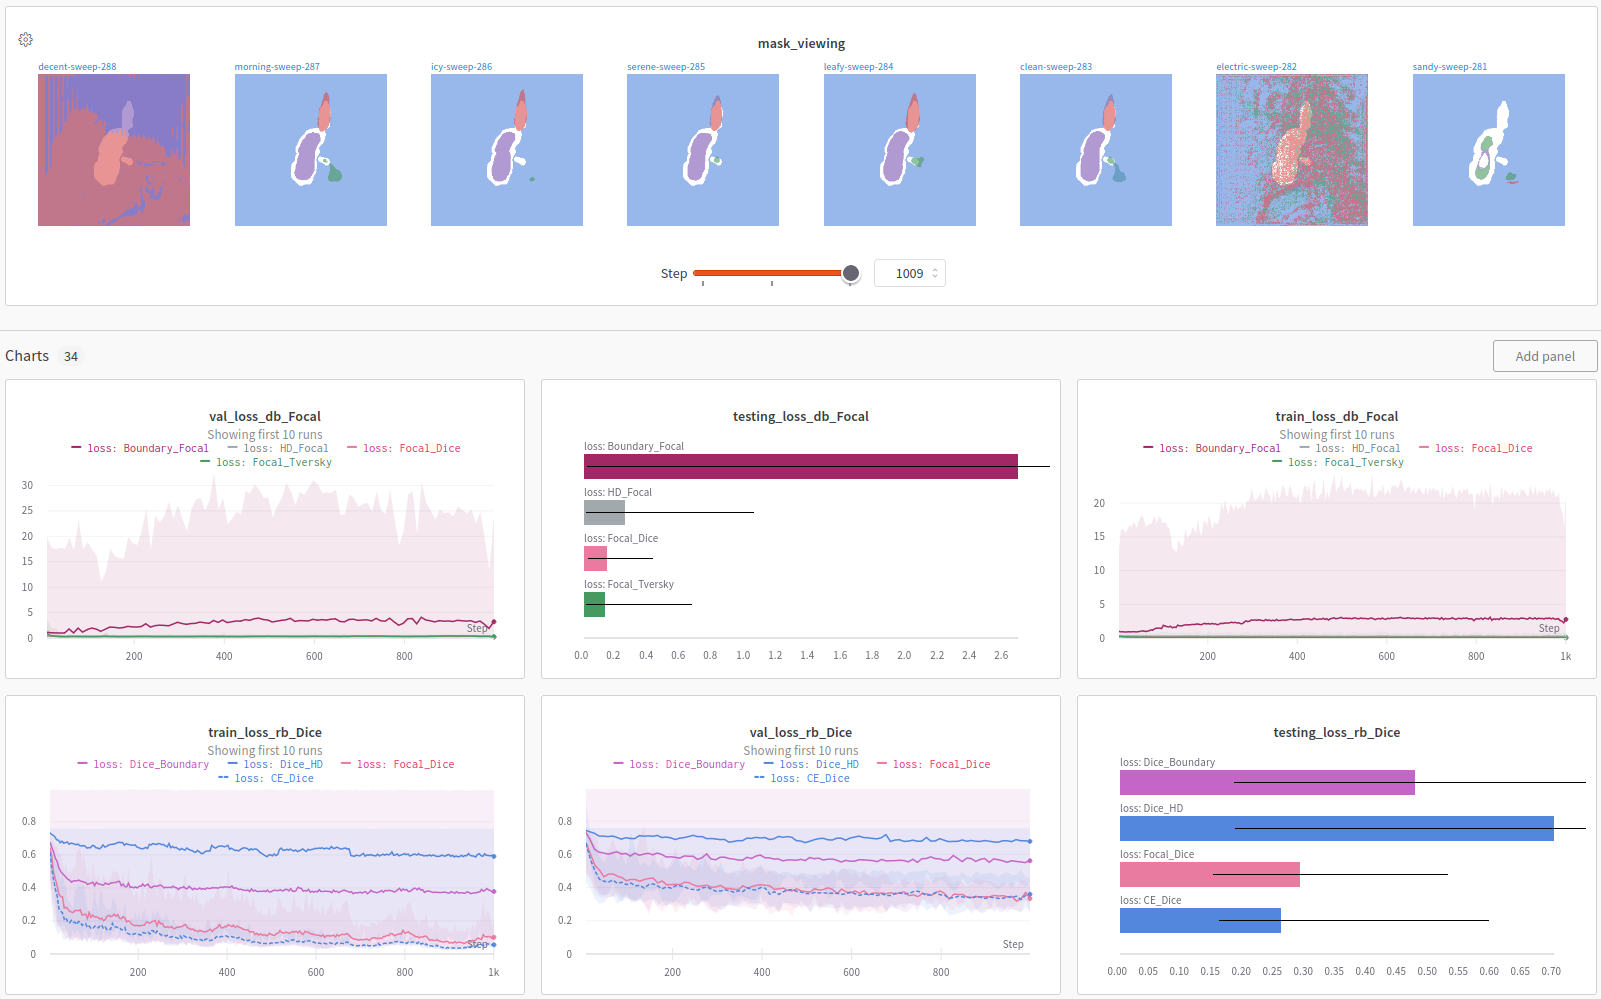
\includegraphics[width=\imgWidthXL]{images/wandb.png}
  \caption[Weights and Biases]{Graphical user interface of \acf{wandb}. The mask viewing section displays predicted masks against the inverted ground truth label. The charts section provides training, validation, and testing results, which can be monitored in real-time.}
  \label{wandb}
\end{figure}
\section{Network Architecture}
\label{sec:network_architecture}
\subsection{U-Net Implementation}
\label{subsec:unet_implementation}
The implemented network architecture is based on the U-Net, introduced in \secref{subsec:segmentation_architectures} as part of an encoder-decoder network. The specific implementation used for this project was obtained from the GitHub repository of Boris Dayma, available at \href{https://github.com/borisdayma/lightning-kitti}{https://github.com/borisdayma/lightning-kitti} and is described in the appendix in \secref{sec:unet} in more detail. 

\subsection{Integration of Loss Functions}
\label{subsec:integration_loss_functions}
Each loss function is structured as a separate class and imported during the model initialization. During the training process, the forward function of the corresponding loss function class is utilized to compute the loss.

For instance, the deep learning class is implemented as follows:
\lstdefinestyle{mystyle}{
    language=Python,
    backgroundcolor=\color{black},
    basicstyle=\color{white}\ttfamily\small,
    keywordstyle=\color{rwuvioletlight},
    numberstyle=\tiny\color{gray},
    stringstyle=\color{rwuvioletlight},
    commentstyle=\color{rwucyanlight},
    morecomment=[l]{\#},
    breakatwhitespace=false,
    breaklines=true,
    captionpos=b,
    keepspaces=true,
    numbers=left,
    numbersep=5pt,
    showspaces=false,
    showstringspaces=false,
    showtabs=false,
    tabsize=2,
    emph={view,size,sum,mean}, % list your function names here
    emphstyle=\color{rwucyan40}\bfseries % set the style for function names
}
\begin{lstlisting}[style=mystyle, caption={Implementation of the Dice Loss function for semantic segmentation tasks, inheriting from PyTorch's \texttt{nn.Module} class. The function calculates the loss based on predicted and ground truth tensors. The tensors are reshaped, and the intersection and cardinality of the predictions and ground truth are calculated. The dice score is computed, and the loss is returned as the mean of 1-\ac{DSC}. The implementation allows including or excluding the background class in the loss calculation, providing flexibility for various segmentation scenarios. The required dependencies are \texttt{torch} and \texttt{torch.nn}.}]
  import torch
  import torch.nn as nn
  
  class DiceLoss(nn.Module):
      def __init__(self, eps=1e-6, do_bg=True) -> None:
          super(DiceLoss, self).__init__()
          self.eps = eps
          self.do_bg = do_bg
  
      def forward(self, y_hat: torch.Tensor, y: torch.Tensor):
          bs, cl = y.size(0), y.size(1)
          y, y_hat = y.view(bs, cl, -1), y_hat.view(bs, cl, -1)
          intersec = torch.sum(y_hat * y, dim=(0, 2))
          card = torch.sum(y_hat + y, dim=(0, 2))
          diceScore = (2 * intersec + self.eps) / (card + self.eps)
          if(self.do_bg==False):
            dice_score=dice_score[1:, ...]
          return (1. - dice_score).mean()
  \end{lstlisting}
Other loss functions in this work follow a similar structure to the deep learning class, ensuring a consistent and modular approach to handling various loss functions during model training.
\section{Image Analysis Spreadsheet}
\label{sec:image_analysis_spreadsheet}
\begin{figure}[H]%[htbp]
  \centering
  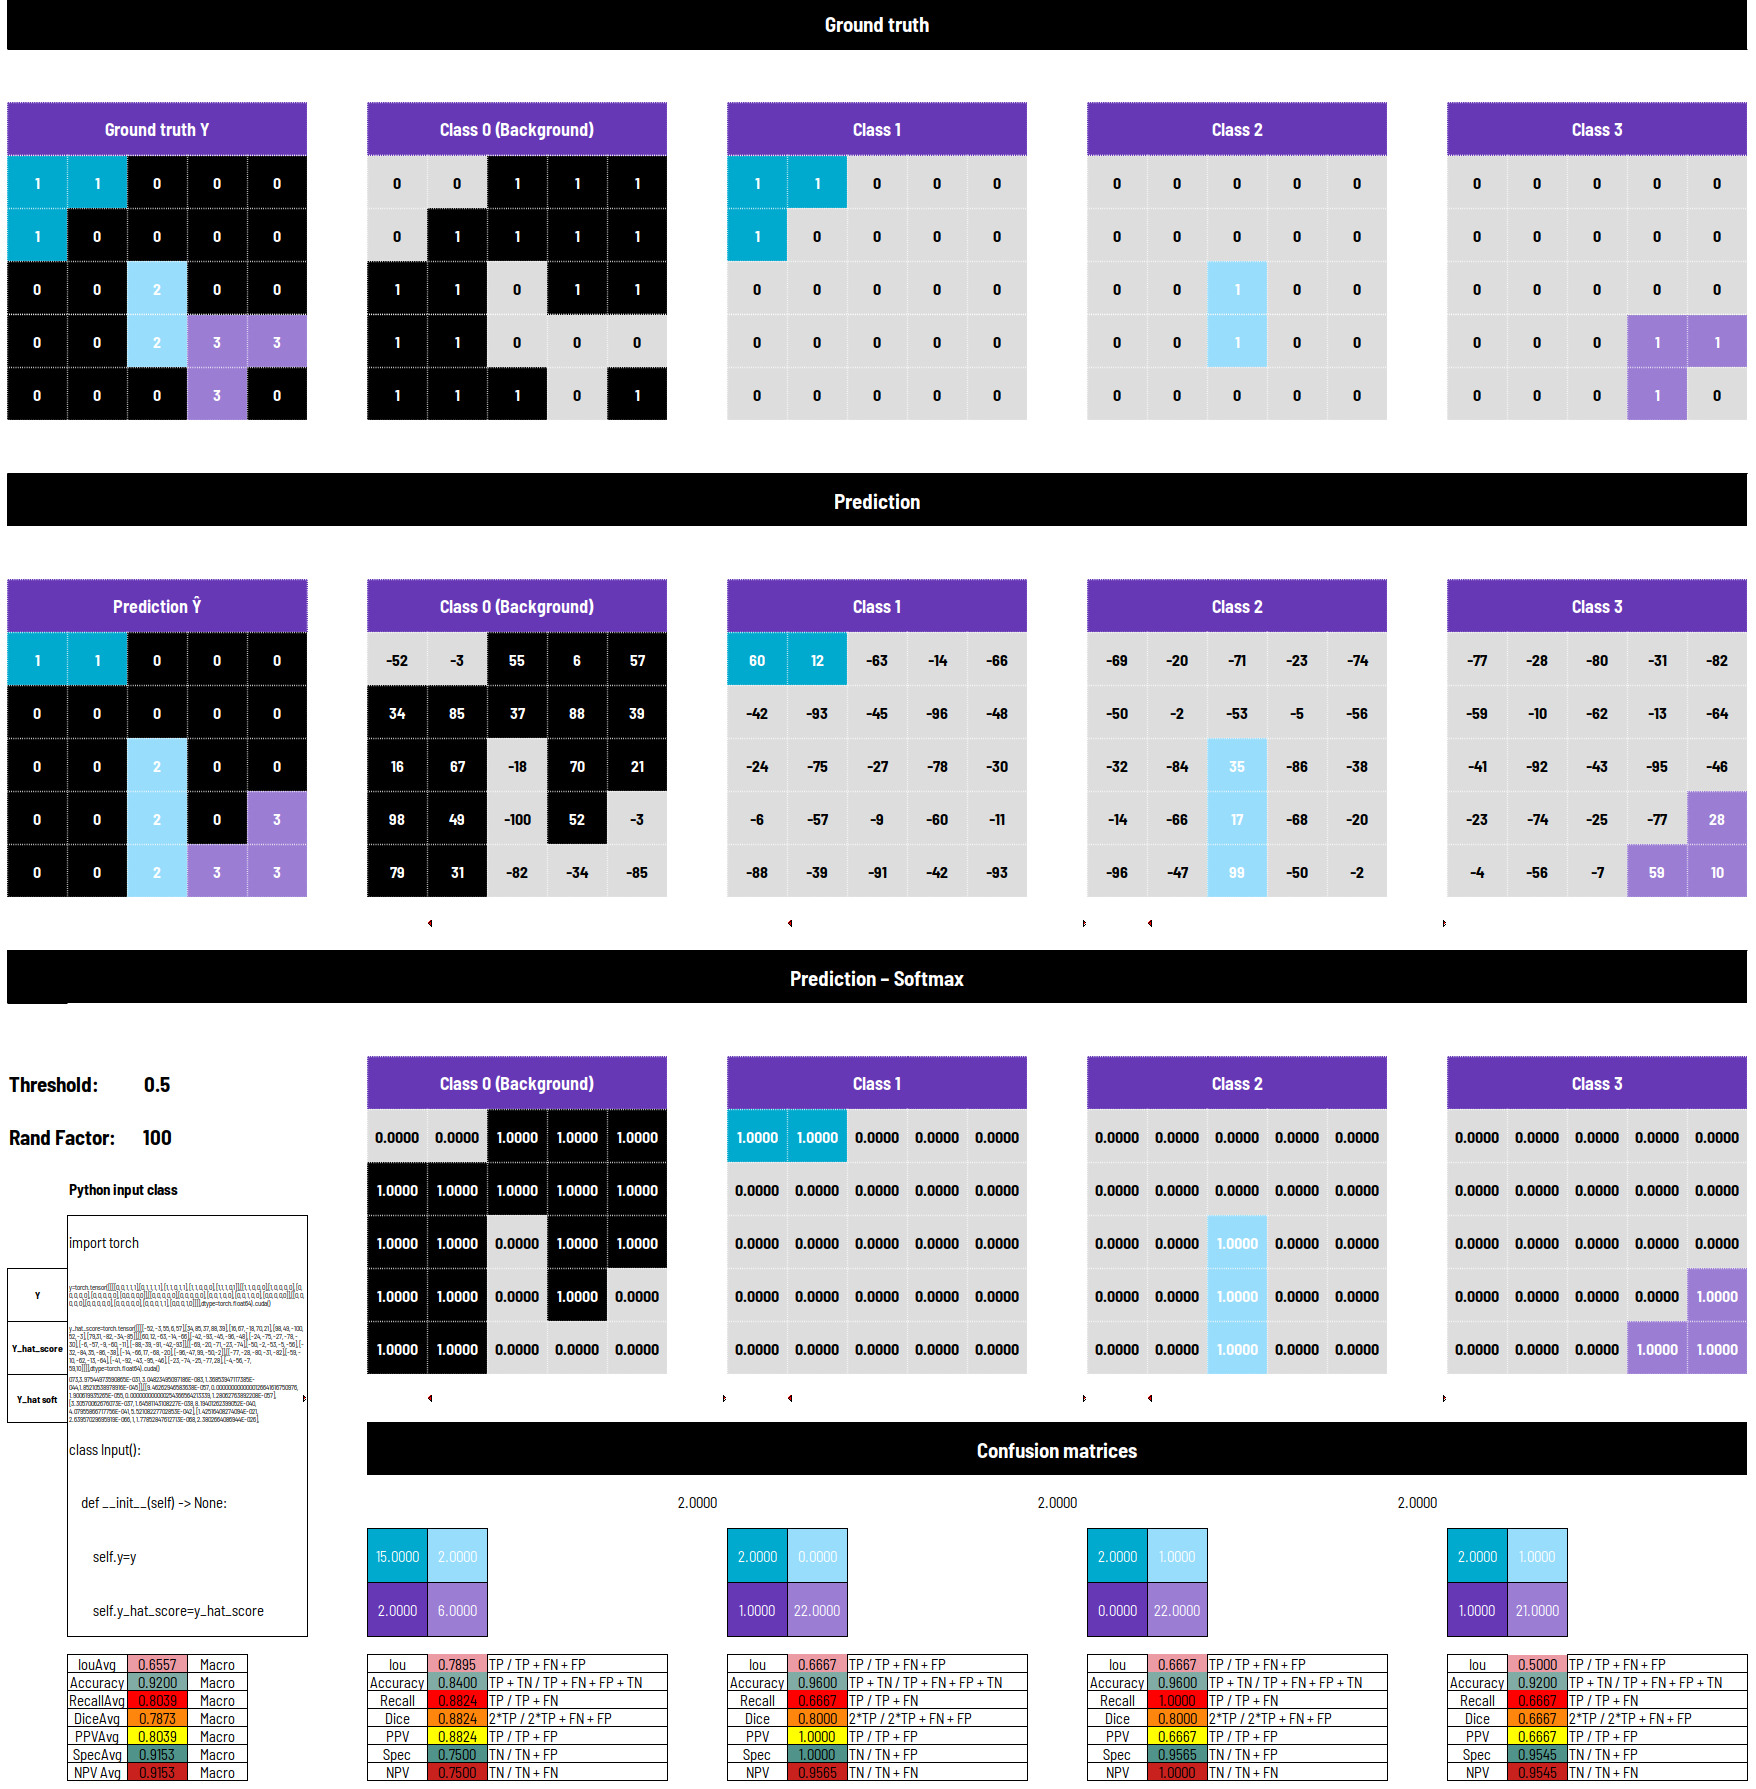
\includegraphics[width=\imgWidthXL]{images/workstation.png}
  \caption[Image Analysis Spreadsheet]{The screenshot showcases a set of (5,5) sized images. The top row displays the ground truth, the second row presents the corresponding prediction scores, and the third row illustrates the application of the softmax function on the predictions as defined in \secref{sec:softmax}. Beneath these toy images, the corresponding metrics are calculated based on the confusion matrices.}
  \label{workstation}
\end{figure}
In addition to the standard libraries and frameworks, a unique working environment using LibreOffice Calc was set up. This allowed for a more in-depth analysis of loss functions at the pixel level. An environment for small images of size (5,5) and (10,10) with up to four classes were created for ground truth labels, prediction scores, and softmax probabilities. The spreadsheet further calculates the confusion matrix of each class and the seven metrics introduced in \secref{subsec:segmentation_metrics}. The Calc spreadsheet organized the images to visualize and manipulate the data quickly. The spreadsheet was further connected to a Python script, which interfaced with the deep learning framework to compute and analyze the various losses. This custom setup allowed to gain deeper insights into the behavior and effectiveness of different loss functions and metrics on a small scale. It helped to understand their impact on semantic segmentation performance better.
